
\section{\label{app:gravity} Modifications for a Spherical Self-Gravitating Star}

In papers II and III, we calculated the hydrostatic expansion of the base state
in plane-parallel geometry under the assumption that the weight of the
material above (or below) any given fluid parcel does not change
during hydrostatic expansion.  This assumption holds when the
gravitational acceleration is independent of location.  Here we discuss the
modifications to the algorithm in paper III required to treat a spherical 
self-gravitating star.

\subsection{One-dimensional Results}

To test the spherical base state expansions, we inject heat at a
steady rate into a one-dimensional white dwarf model.  This is similar
to the first test in paper II, except now in spherical coordinates.
As in that test, the compressible method with which we compare the low Mach number method 
is the FLASH code's implementation of the
piecewise-parabolic method (PPM) in a one-dimensional spherical geometry.  
The initial conditions for the white dwarf are those described in
Section 4.1 of paper III for the central region.

%A simple initial model for a white dwarf was constructed by specifying
%a central density of $2.6\times 10^9~\gcc$, a central temperature of
%$7\times 10^8$~K, and a composition of 30\% carbon and 70\% oxygen,
%and integrating the equation of hydrostatic equilibrium outward (using
%spherically symmetric self-gravity) while constraining the entropy to
%be constant.  Once the temperature of the model falls to $10^7$~K, it
%is held constant---this happens only at the very outer region of the
%star.  Together with the equation of state, this completely determines
%the density, temperature, and pressure structure of the star.

In the expansion of a plane-parallel atmosphere, heating at a
height $r$ above the base does not affect the pressure or density 
below that height.  By contrast, in a spherical symmetric
self-gravitating star, heating at a radius $r$ will lead to a pressure
and density decrease at the center in addition to the expansion of the
outer layers (see Schwarzchild \& Harm, 1965, ApJ, 146, 855).


We apply a heating function of the form:
\begin{equation}
\Hext = H_0 \exp \left [-(r-r_0)^2 / W^2 \right ] \enskip ,
\end{equation}
with $r_0 = 4\times 10^7$~cm, $W = 10^7$~cm, and $H_0 = 1\times
10^{16}$~erg~g$^{-1}$~s$^{-1}$. This is the same functional form as used
in the first test of paper II, but with a lower amplitude.  Still, this
heating rate is far higher than what is expected during the convective
phase of Type Ia SNe.  The heating term is added to the enthalpy
equation in the low Mach number equations in the same fashion as
described in paper II.  In this test, we do not consider reactions.
Since this is a one-dimensional test all perturbational quantities,
as well as $\Ubt,$ are zero, so we are directly testing the computation of 
$w_0$ as and the base state update as described in
the {\bf Advect Base} procedure defined above.  
Both the PPM and low Mach calculation use 768 zones in a domain $5\times
10^8$~cm high.

Figure~\ref{fig:spherical768} shows the structure of the star after
heating for 10~s.  The gray line is the initial star before any
heating.  
%The solid black line is the PPM result and the dotted and
%dashed lines are the low Mach number model with advective CFL numbers
%of $0.5$ and $0.1$ respectively (the PPM calculation used a CFL number
%of $0.5$).  
We see that the compressible and low Mach number models
agree extremely well.  Both capture the decrease in the density and
pressure at the center of the star and the considerable expansion in
radius.  Only at the surface of the star do the temperatures differ slightly.
In all calculations, we set the minimum temperature to $5\times
10^6$~K.  The PPM simulation required 13488 steps and the low Mach
(CFL $=0.5$) calculation needed 203.  Over the course of the
simulation, the Mach number of the flow remained less than $0.35$, with the
maximum Mach number occurring at the surface of the star.  This Mach
number pushes the limits of validity of the low Mach number model;  a
smaller perturbation amplitude would result in a smaller Mach number.

Future improvements to the overall spherical base-state adjustment
algorithm will address the expansion in a simulation where the medium
outside the star is not brought down to arbitrarily low densities, but
instead a ``cutoff density'' is applied, as in the case of the
plane-parallel results presented in this paper. However, we expect
the changes to the overall method shown here to be small. \MarginPar{new}

{\color{red} Add a figure showing that we retain the correct solution 
even when we place higher density material outside the star.}


\clearpage

\begin{figure*}
\begin{center}
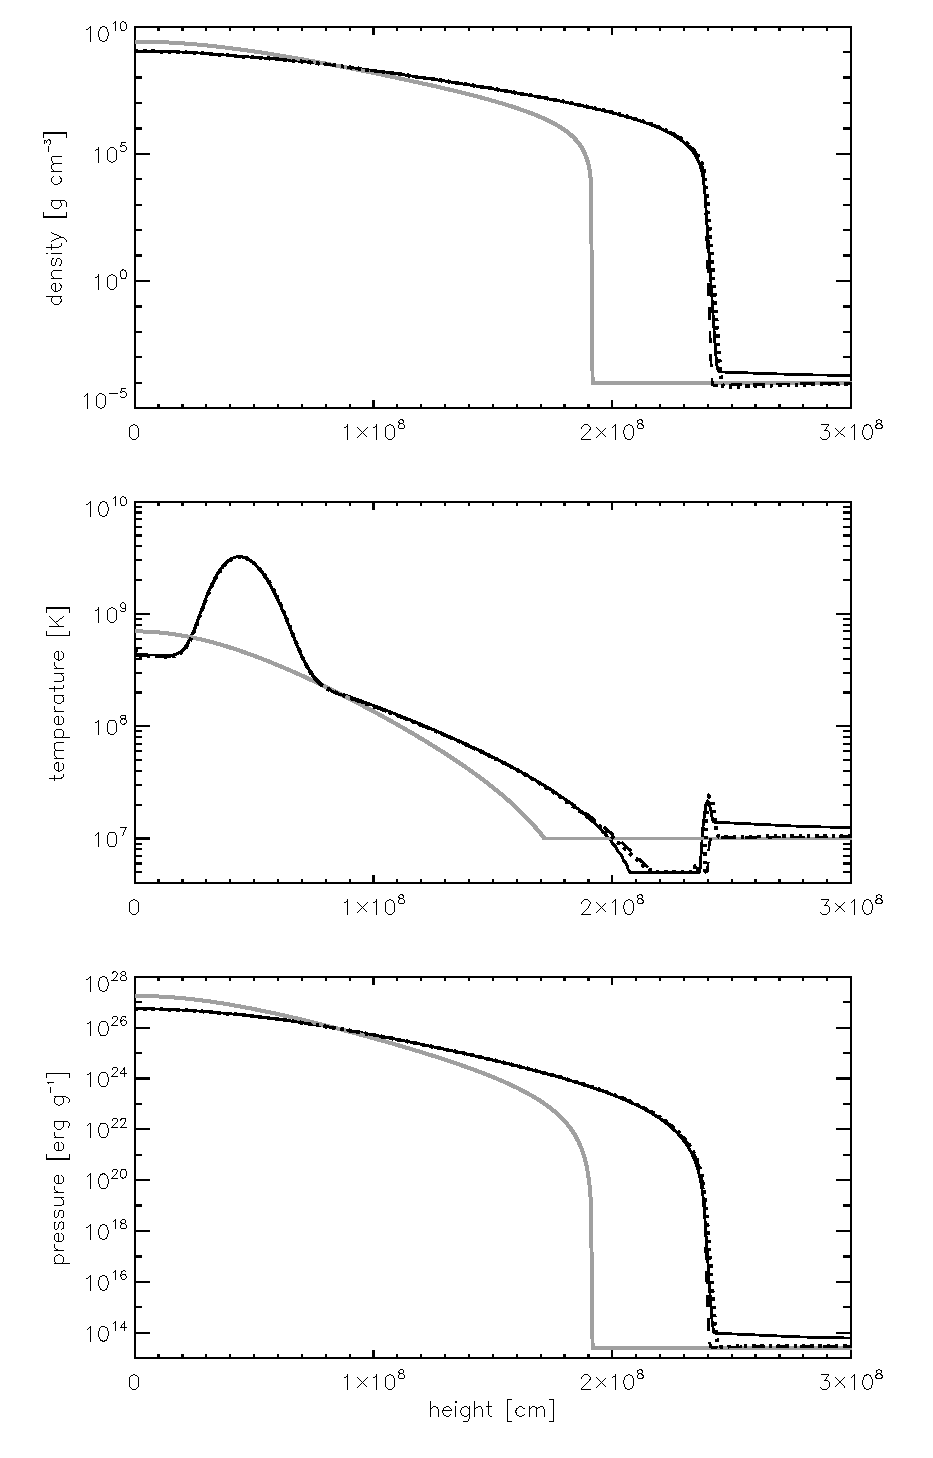
\includegraphics[width=5.0in]{\sphericalfigpath/spherical_adjust_768}
\end{center}
\caption{\label{fig:spherical768} Hydrostatic adjustment of a
spherically symmetric white dwarf with self-gravity.  The gray line
represents the initial model;  all other lines are after 10~s of heating.
The solid black line is the fully compressible solution, the dotted line is the
low Mach number solution with a CFL number of 0.5,  and the dashed line is
the low Mach number solution with a CFL number of 0.1.  All
simulations used 768 equally spaced zones.  We see excellent agreement
between the compressible and low Mach number models.  The only
differences appear at the top of the atmosphere, where the outer
boundary condition can influence the results.}
\end{figure*}


\end{document}

